\section{DNS \cite{reddy2020,dubey2022,dubey2023}}
The Deep Noise Suppression challenge is a yearly challenge organized by Microsoft Research. The first challenge was introduced in 2020, and it has been held annually since. If focuses specially on Speech Enhancement tasks and real-time settings. The Deep Noise Suppression (DNS) challenge aims to unify research activity in the Speech Enhancement domain by making the train/test datasets and subjective assessment system available to the public. It releases a large clean speech and noise datasets. It also provides configurable synthetization scripts for producing the training datasets. It also releases a part of the test dataset.

\subsection{DNS 2020 \cite{reddy2020}}
\subsubsection{Clean Dataset}
The clean speech dataset is obtained from Librivox, which is a public audiobooks dataset. It has the audiobooks recordings of over 10000 public domain books in multiple languages, the majority of which are in English \cite{panayotov2015}. Although most of these recordings were of excellent speech conditions and quality, it had many recordings with poor conditions such as speech distortion, background noise, and reverberation. These poor-conditioned recordings needed to be removed, as the clean dataset must be free of noisy and poor-conditioned recordings. An online subjective test framework ITU-T P.808 was used to keep only excellent quality recordings. Mean Opinion Score (MOS) was used as a metric by keeping only the upper quartile with respect to MOS. The final clean dataset included 500 hours of speech from 2150 speakers. The filtered clips are then divided into 10-second segments.
\subsubsection{Noise Dataset}
The noise dataset was selected from Audioset \cite{gemmeke2017} and Freesound. Audioset consists of 2 million sound clips of 10s each, where each sound clip is human-labelled. These clips are extracted from YouTube videos belonging to about 600 audio events. Some classes are overrepresented compared to others. A sampling approach was executed to balance each class by having at least 500 clips. Speech activity detector was used to remove any clips containing speech activity. The resulting dataset contained about 150 classes and 60000 clips. Additional 10000 noise clips related to VoIP applications were downloaded from Freesound and DEMAND dataset \cite{thiemann2013}.
\subsubsection{Noisy Dataset}
The noisy dataset is the addition of clean speech from the clean dataset and a noise clip from the noise dataset at various SNR levels. The SNR is only computed using active segments of both the clean and noise signals. This was done to avoid the overshoot of amplitude in impulsive noise (i.e., door shutting or dog barking).

\subsection{DNS 2022 \cite{dubey2022}}
This Deep Noise Suppression (DNS) Challenge was the 4th DNS challenge. The original authors open-sourced the datasets and test sets for reaseachers to train their deep noise suppersion models as well as as a subject evaluation framework based on ITU-Y P.835 to rate and rank-order the challenge entries. In this challenge specifically a new changes was introduced: (i) included mobile devices scenarios in the blind test set;  (ii) Included a personalized noise sup- pression track with baseline; (iii) Added WAcc as an objective met- ric; (iv) Included DNSMOS P.835; (v) Made the training datasets and test sets fullband (48 kHz).
\subsubsection{Clean Dataset}
The clean speech datast consist of six languages, namely English, French, German, Italian, Russian, and Spanish. English clean speech consist of read speech and singing, while the rest of the languages only have read speech. The original authors combined all audio clips form each unique talker into a single file. The PDNS training data has a total of 3,230 talkers, out of which 60\% of the talkerrs are randomly chosen to be the primary talkers while the rest are neighboring talkers. and they also provide the file list for PDNS clean speech with 'primary' and 'secondary' tags, sampling 60\% of the speakers as primary talkers, ensuring a uniform distribu- tion among all languages, read speech or singing.
English speech was derived from Librivox like previous versions mentioned above. English singing data consists of high-quality audio recordings from professional singers contained in the VocalSet corpus.
It has 10.1 hours of clean singing from 20 singers: 9 males and 11 females.
The PDNS English clean speech contains 1934 talkers from Librivox, 110 talkers from VCTK corpus, 20 talkers from Vocalset. The PDNS clean speech consists of 47 talkers for French, 874 for German, 14 for Italian, 7 for Russian, and 224 for Spanish.
\subsubsection{Noise Datatset}
\begin{figure} [H]
    \centering
    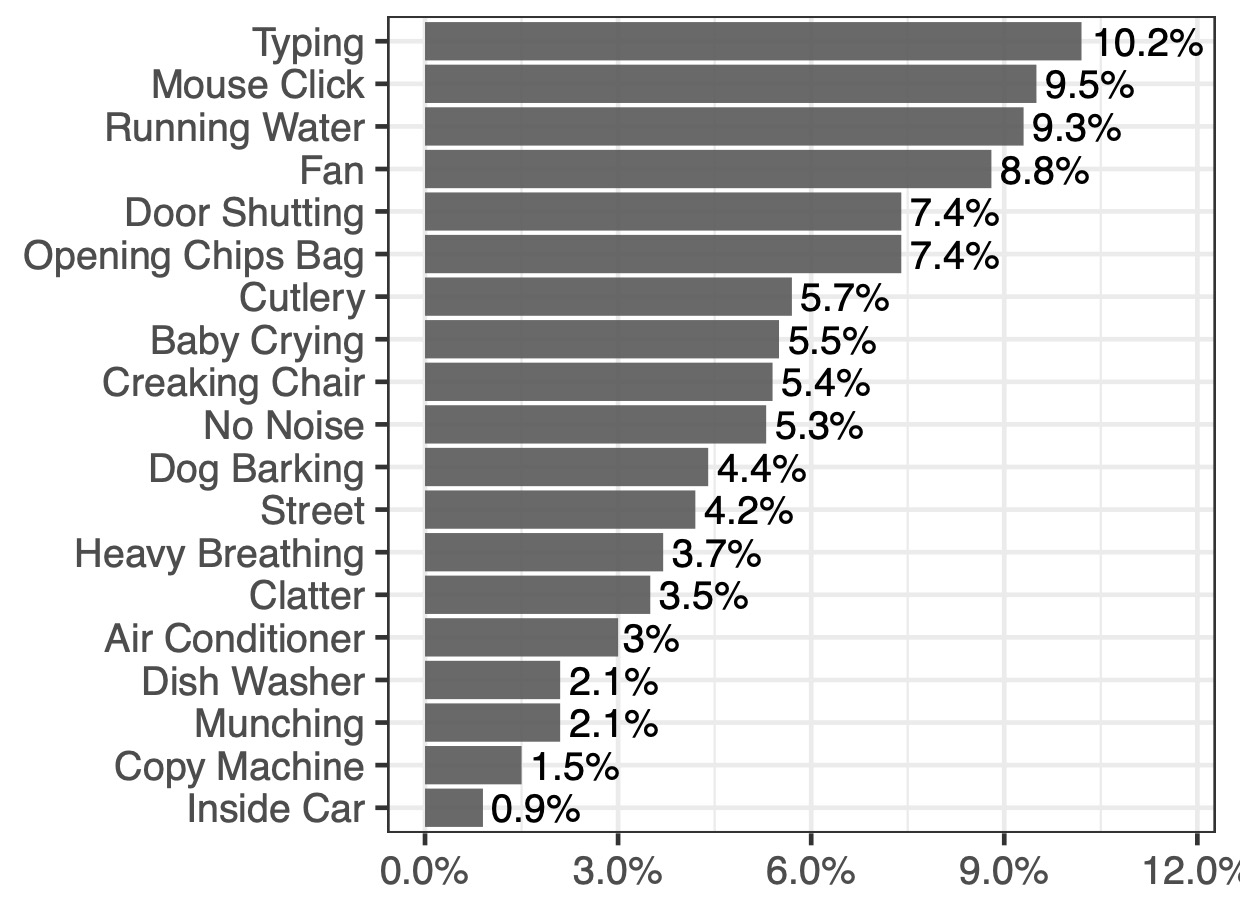
\includegraphics[width=0.75\linewidth]{images/datasets/dns2022-noise.jpg}
    \caption{Distribution of noise types in our blind test set.}
    \label{fig:dns22noise}
\end{figure}
Noise data consists of about 62,000 clips belonging to 150 noise classes.
Audio Set is a
collection of about 2 million human-labeled 10s sound clips drawn from YouTube videos belonging to about 600 audio events.
Approximately 42\% of the clips have a single class, but the rest may have 2 to 15 labels.
The authors used a speech activity detector to remove the clips with any kind of speech activity (voice content) from our noise clips.
The total noise data constitute 181 hours of audio. Fig. \ref{fig:dns22noise} shows the histogram of noise classes included in the blind test set. These noise types were validated by a human listener after the collection of the blind set

\subsubsection{Impulse Response}
They offered over 60,000 synthetic and 248 real room impulse responses, which can be used to create training data with reverberant noise. Depending on the setup selected, the training data synthesiser adds noise to reverberant clean speech. For their DNS models, participants can select between training clean speech and reverberant speech.

\subsection{DNS 2023 \cite{dubey2023}}